Bei hochenergetischen Photonen kann ein $e^-e^+-$Paar erzeugt werden:

\[\gamma + \text{Atomkern} \longrightarrow e^+ + e^- +  \text{Atomkern} \]

\[\gamma + e^- \longrightarrow e^+ + e^- +  e^- \]

Aus Gründen der Impulserhaltung ist dieser Prozess nur im Coulombfeld eines Stoßpartners möglich,
welcher den Rückstoß aufnimmt. Dabei kann es sich entweder um einen Atomkern oder um ein
Hüllenelektron handeln, wobei eine Reaktion mit letzterem stark unterdrückt ist. 
\\
Die minimale Energie für eine Paarerzeugung ist

\[ E_\gamma \geq 2m_ec^2 > 1{,}022\,\text{MeV}. \]

Bei hohen Energie dominiert die Paarerzeugung. Die Feynmangraphen niedrigster Ordnung sind:

\begin{figure}[H]
	\centering
	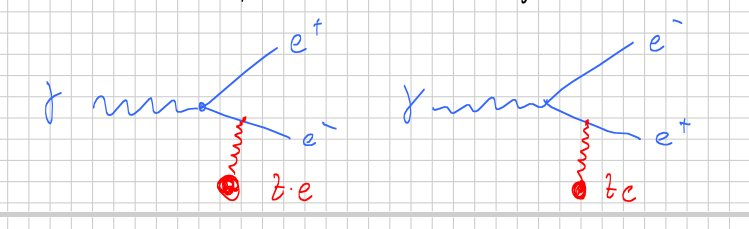
\includegraphics[width=0.5\textwidth]{fgraph2.jpg}
	\caption{	 ???}
	\label{fgraph2}
\end{figure}

Die Berechnung der Paarerzeugung ist analog zur Bremsstrahlung ("`Crossing-Symmetrie"'). Der
Wirkungsquerschnitt steigt mit größerer Photonenergie stark an und erreicht schließlich einen
asymptotischen Wert. Die Wechselwirkungswahrscheinlichkeit hängt also von der Photonenergie ab:

\begin{itemize}
  \item \textbf{niederenergietische Photonen}\\
  Das Photon muss dem Atomkern sehr nahe kommen, um eine Paarerzeugung zu ermöglichen; das Photon
  wechselwirkt mit dem "`nackten"' Kern. Wirkungsquerschnitt pro Atom:
  \[\sigma_{\text{Paar,nucl}} = 4\alpha\cdot r_e^2 Z^2
  \left[\frac{7}{9}\,\text{ln}\left(\frac{2E_\gamma}{m_ec^2}-\frac{109}{54} \right) \right]  \]
  für $1< \frac{E_\gamma}{m_ec^2} < \frac{1}{\alpha\cdot Z^{1/3}}$
  \item \textbf{hochenergetische Photonen}\\
  Für sehr hohe Energie des Photons ist Paarerzeugung auch bei großen Stoßparametern möglich. Die
  Abschirmung des Kernfeldes durch Hüllen\-elektronen muss berücksichtigt werden. Der
  Wirkungsquerschnitt pro Atom strebt einem energieunabhängigen Grenzwert zu:
  \[\sigma_{\text{Paar,nucl}} = 4\alpha\cdot r_e^2\cdot Z(Z+1)^*
  \left[\frac{7}{9}\,\text{ln}\left(\frac{183}{Z^{1/3}}-\frac{1}{54} \right) \right]  \]
  für $\frac{E_\gamma}{m_ec^2} > \frac{1}{\alpha\cdot Z^{1/3}}$. Bei $^*$ wird näherungsweise die
  Paarerzeugung im Feld der Hüllenelektronen berücksichtigt.
\end{itemize}

Für den gesamten Wirkungsquerschnitt pro Materialvolumen wird mit der Anzahl der Atome, also
$\frac{N_A\rho}{A}$ multipliziert. Aus dem gesamten Wirkungsquerschnitt kann man die mittlere freie
Weglänge eines hochenergetischen Photons 

\[\lambda_{\text{Paar}} = \frac{A}{N_A\rho}\cdot \frac{1}{\sigma_{\text{Paar,Atom}}} \]

berechnet werden. Ein Vergleich mit der Strahlungslänge ergibt 

\[\lambda_{\text{Paar}} = \frac{9}{7}\cdot \chi_0. \]
